%%%%%%%%%%%%%%%%%%%%%%%%%%%%%%%%%%%%%%%%%%%%%%%%%%%%%%%%%%%%%%%%%%%%%%%%%%%%%%%
% Capítulo 3: Procedimiento experimental 
%%%%%%%%%%%%%%%%%%%%%%%%%%%%%%%%%%%%%%%%%%%%%%%%%%%%%%%%%%%%%%%%%%%%%%%%%%%%%%%

%Este capítulo ha de contar con seccciones para la descripción de los experimentos 
%y del material.

%También debe haber una sección para los resultados obtenidos y una última de 
%análisis de los resultados.

%++++++++++++++++++++++++++++++++++++++++++++++++++++++++++++++++++++++++++++++
\section{Descripción de los experimentos}
\label{3:sec:1}
\parindent=0.5cm
\raggedright
\subsection{Primer experimento}
El experimento llevado a cabo es la realización de la integral definida, la aproximación
mediante la regla del trapecio y la regla del trapecio compuesta. Compararemos los resultados para ver si se obtiene una aproximacón fiable.
 Veamos\\
Integral definida 
\[
\int_{-1}^{1} \frac{1}{\sqrt(2\pi)} \quad\text{e}^{\frac{-x^2}{2}}dx
\]
Regla del Trapecio
\[
\int_{-1}^{} \frac{1}{\sqrt(2\pi)} \quad\text{e}^{\frac{-x^2}{2}}dx\approx\left(1-(-1)\right)\frac{f(-1)+f(1)}{2}
\]
En esta gráfica vemos la función original y el área que va a ser evaluada por la regla del trapecio simple, que coincide con el rectángulo de vértices (-1,0), (-1,0.24197), (1,0.24917)
 y (1,0), habiendo calculado f(1) = f(-1) = 0.24197 .

\includegraphics[width=1.15\textwidth]{images/trasim}

 Regla del Trapecio compuesta con n=4
\[
h=\frac{1-(-1)}{4} =\frac{1}{2} 
\]
\[
\int_{-1}^{1} \frac{1}{\sqrt(2\pi)} \quad\text{e}^{\frac{-x^2}{2}}dx\approx\left[f(-1) + f(\frac{-1}{2}) + f(0) + f(\frac{1}{2}) + f(1)\right]
\]


\subsection{Segundo experimento}
En este experimento vamos a ver los distintos errores que puede tomar el teorema para los posibles resultados de $\epsilon$.
Recordamos que $\epsilon$ pertenecerá al intervalo [a,b], en este caso, el intervalo [-1,1].
Por tanto,

\[
-\frac{\left(1-(-1)\right)^3}{12}  \displaystyle f^{(2)}(\epsilon)

\forall \epsilon \owns [-1,1]
\]


Efectuando la derivada segunda que es necesaria, la ecuación queda:
\[
-\frac{2}{3\sqrt(2\pi)} \quad\text{e}^{\frac{\epsilon^2}{-2}}  \displaystyle  (1-\epsilon^2)

\forall \epsilon \owns [-1,1]
\]



\subsection{Tercer experimento}
En este experimento se comparará la eficiencia del tiempo que se tarda en hallar dos resultados de la integral, en un caso
 por la integración de trapecio simple y en el otro caso por la integración de trapecio compuesta. El programa empleado para
ello nos permitirá repetir el experimento tantas veces como deseemos y de esta manera se podrá sacar un porcentaje de error entre un tiempo 
y otro.



%++++++++++++++++++++++++++++++++++++++++++++++++++++++++++++++++++++++++++++++
\section{Descripción del material}
\label{3:sec:2}
\parindent=0.2cm
\raggedright
El material que hemos empleado para la realización de este proyecto es el lenguaje de
programación Python(versión 2.7.3.), para la creación de los programas que verifican este método de integración, 
y el sistema de composición de textos \LaTeX para el diseño del proyecto, todo ello efectuado en el sistema operativo
Bardinux (Linux).


%++++++++++++++++++++++++++++++++++++++++++++++++++++++++++++++++++++++++++++++
\section{Resultados obtenidos}
\label{3:sec:3}
\parindent=0.2cm
\raggedright
\subsection{Resultados del primer experimento}
Los resultados obtenidos son:
Integral definida 
\[
\int_{-1}^{1} \frac{1}{\sqrt(2\pi)} \quad\text{e}^{\frac{-x^2}{2}}dx\approx0.682689 
\]
Regla del Trapecio
\[
\int_{-1}^{1} \frac{1}{\sqrt(2\pi)} \quad\text{e}^{\frac{-x^2}{2}}dx\approx\left(1-(-1)\right)\frac{f(-1)+f(1)}{2}=0.483941
\]
Regla del Trapecio compuesta con n=4
\[
\int_{-1}^{1} \frac{1}{\sqrt(2\pi)} \quad\text{e}^{\frac{-x^2}{2}}dx\approx\left[f(-1) + f(\frac-{1}{2}) + f(0) + f(\frac{1}{2} + f(1)\right]\approx0.672435
\]
\subsection{Resultados del segundo experimento}
Tomando varios valores de $\epsilon$,obtenemos la siguinte gráfica:








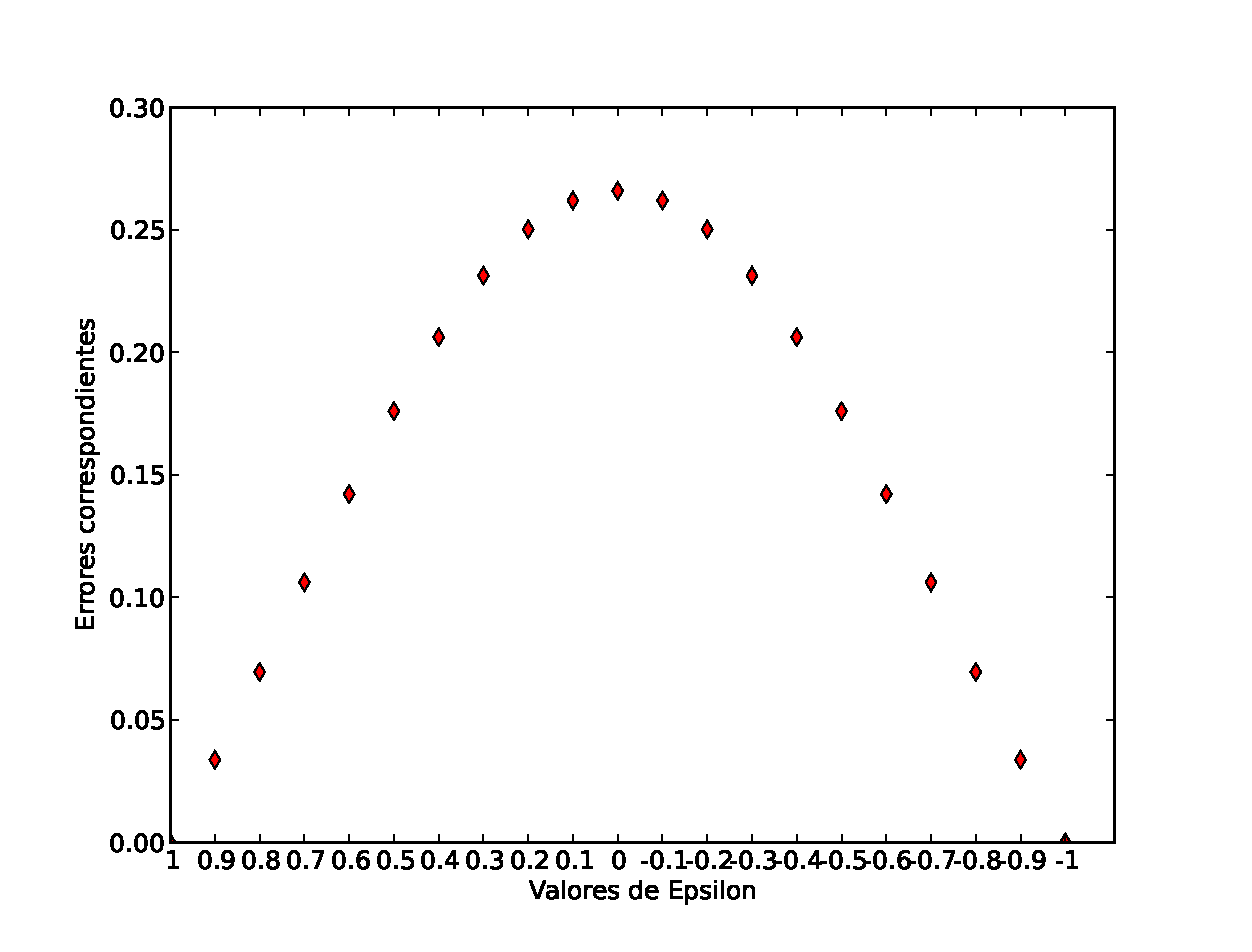
\includegraphics[width=1\textwidth]{images/imgraf}

Algunos valores representativos son:

$\epsilon$=1$\Rightarrow$ Error=0

$\epsilon$=0$\Rightarrow$ Error=0.26596

\subsection{Resultado del tercer experimento}

En la siguiente gráfica vemos un ejemplo de uno de los experimentos:

%------------------------------------------------------------
%\begin{figure}[!th]
%\begin{center}
%\includegraphics[width=0.75\textwidth]{images/figura1.eps}
%\caption{Ejemplo de figura}
%\label{fig:1}
%\end{center}
%\end{figure}
%------------------------------------------------------------------------------
Resultados del tiempo empleado para la regla del trapecio simple y la regla del trapecio compuesta
%--------------------------------------------------------------------------
\begin{table}[!ht]
\begin{center}
\begin{tabular}{|c|c|} \hline 
\textbf{Tiempo por Trapecio simple} & \textbf{Tiempo por trapecio compuesto} \\ 
\textbf{(en s)} & \textbf{(en s)} \\ \hline \hline
0.1412169 &
0.1414737
\\
\hline

0.1414649 &
0.1415798
\\
\hline

0.1412210 &
0.1413900
\\
\hline


\end{tabular}
\end{center}
\caption{Resultados experimentales de tiempo (s) y velocidad (m/s)}
\label{tab:1}
\end{table}



cuyo porcentaje de error del trapecio compuesto con respecto al simple fue de 99.9668.
El experimento se ejecutó varias veces y con distinto número de divisiones para la regla del trapecio compuesto,
para interpretar los diferentes comportamientos del tiempo empleado. En el siguiente apartado se analizarán dichos comportamientos.

%------------------------------------------------------------------------------

%++++++++++++++++++++++++++++++++++++++++++++++++++++++++++++++++++++++++++++++
\section{Análisis de los resultados}
\label{3:sec:4}
\parindent=1cm
\raggedright
 En el primer experimento, en el cual comparábamos los distintos resultados según usáramos los métodos de integración,
 observamos que la integral definida tiene como resultado 0.682689; la integración por la regla del trapecio simple, 0.483941;
 y la integración por la regla del trapecio compuesta, 0.672435.
Así pues, obtenemos un error de 0.1978748 en la regla del trapecio simple y un error de 0.010254 en la regla del trapecio compuesta.
Podemos ver claramente que la regla del trapecio compuesta es más exacta que la regla del trapecio simple, si bien sigue sin ser del todo exacta.
Esto tiene sentido con lo llevado a cabo en el segundo experimento, ya que el error máximo encontrado, según el error que se nos daba en la regla del trapecio,
es de 0.26596. Analizando dicho experimento, vemos un patrón que sigue la función del error, que varía según $\epsilon$.
Si derivamos esta función e igualamos a cero, obtendremos los valores máximos y mínimos de error. Esto es,

\[
\quad\text{e}^{\frac{-\epsilon^2}{2}} \displaystyle (1-\epsilon) \displaystyle \epsilon = 0
\]

Se ve fácilmente que ni el primer múltiplo ni el segundo tiene solución si se igualan a cero, así que la única solución a esa ecuación es $\epsilon$ = 0.
Su correspondiente error, que será el máximo, es de 0.26596.

En el tercer experimento, al comparar los tiempos de ejecución, hemos visto que a mayor número de divisiones en el método del trapecio compuesto, eran mayores las diferencias
 de tiempo, y por tanto el porcentaje, como es lógico. 

